\RequirePackage{docswitch}
\setjournal{\flag}

\documentclass[\docopts]{\docclass}


\usepackage{lsstdesc_macros}

\usepackage{xspace}
\usepackage{graphicx}
\graphicspath{{./}{./figures/}{.logos}}
\bibliographystyle{apj}


\newcommand{\textul}{\underline}
\newcommand{\qp}{\texttt{qp}}
\newcommand{\pz}{photo-$z$ PDF}
\newcommand{\Pz}{Photo-$z$ PDF}
\newcommand{\mgdata}{bright\xspace}
\newcommand{\Mgdata}{Bright\xspace}
\newcommand{\ssdata}{faint\xspace}
\newcommand{\Ssdata}{Faint\xspace}


\begin{document}

\title{ Approximating photo-z PDFs for large surveys }


\begin{abstract}

Upcoming and ongoing galaxy surveys will and do produce redshift probability 
distribution functions (PDFs) in addition to traditional photometric redshift 
(photo-$z$) point estimates.
However, the storage of \pz s may present a challenge with increasingly large 
catalogs, as we face a trade-off between the accuracy of subsequent science 
measurements and the storage cost.
This paper presents \qp, a Python package facilitating manipulation of 
approximations of 1-dimensional PDFs, as suitable for \pz s.
We use \qp\ to investigate the performance of three simple PDF storage formats 
on two realistic mock datasets, representative of upcoming surveys with 
different data qualities, as a function of the number of stored parameters per 
\pz, using metrics of both individual \pz s and an estimator of the overall 
redshift distribution function.

\end{abstract}

\dockeys{methods: data analysis, catalogs, surveys}

\maketitlepost





\section{Introduction}
\label{sec:intro}


Ongoing and upcoming wide-field imaging surveys such as the Large Synoptic 
Survey Telescope 
(LSST)\footnote{\url{https://www.lsst.org/}}\citep{ivezic_lsst:_2008} will 
observe billions of galaxies photometrically, without follow-up spectroscopy.
Studies of precision cosmology and galaxy evolution with these data will thus 
rely almost exclusively on the method of photometric redshift (photo-$z$) 
estimation.
Photo-$z$s are subject to a number of systematic errors, some caused by the 
estimation procedures and others intrinsic to the data itself.
The photo-$z$ community has come to favor methods that provide a redshift 
probability distribution function (PDF) that includes information about the 
potential for such systematic errors for each galaxy in the survey.

Given the tremendous size of the surveys in question, storage of these 
probability distributions involves making difficult decisions.
Each survey seeks to balance accuracy against storage cost in creating a 
catalog of \pz s made available to the scientific community.
For example, the \pz\ catalog that LSST will release will be limited to 
$\sim100$ floating point numbers per galaxy\citet[section 
4.2.2]{juric_data_2017}, with plans to store \pz s derived by multiple methods.
The problem of \pz\ approximation for large surveys was first addressed in 
\citet{carrasco_kind_sparse_2014} in the context of a single galaxy survey, a 
limited set of \pz\ approximation schemes, and metrics appropriate for 
deterministic, not probabilistic, objects.
However, we expect the choice of \pz\ approximation, and the number of stored 
parameters associated with it, will depend on the science case and its 
requirements on \pz\ accuracy: different science cases will need different 
accuracy metrics.
In this paper, we address the question of \textit{how} these choices should be 
made in general, by providing the publicly available \qp\ Python 
package\footnote{\url{https://github.com/aimalz/qp}} to enable each survey to 
optimize their \pz\ approximation via mathematically motivated and 
science-driven metrics.
We demonstrate this approach on two sets of realistic mock data.

In Section~\ref{sec:methods}, we outline how \qp\ can be used to optimize the 
choice of \pz\ parametrization.
In Section~\ref{sec:data}, we describe the mock datasets on which we perform 
such an analysis.
We present the results of this procedure in Section~\ref{sec:results} and make 
recommendations for the use of \qp\ by the photo-$z$ community in 
Section~\ref{sec:conclusions}.

\section{Methods}
\label{sec:methods}


We have developed the \qp\ Python package to facilitate the parametrization and 
approximation of \pz s.
A \texttt{qp.PDF} object can carry a number of different parametrizations, each 
associated with a representation.
Conversions between parametrizations are facilitated by the 
\texttt{numpy}\footnote{\url{http://www.numpy.org/}}, \texttt{scipy} 
\footnote{\url{https://www.scipy.org/}}, and 
\texttt{scikit-learn}\footnote{\url{http://scikit-learn.org}} 
\citep{pedregosa_scikit-learn:_2011} tools.
The currently supported parametrizations are described in 
Section~\ref{sec:approx}.
The \qp\ package also provides a few built-in metrics of the accuracy of a 
representation of a \pz\ relative to a given parametrization that has been 
designated as the reference representation.
Built-in plots are made using 
\texttt{matplotlib}\footnote{\url{https://matplotlib.org/}}.
The currently implemented metrics are described in Section~\ref{sec:metric}.
Large-scale tests can be conducted using the \texttt{qp.Ensemble} class that 
provides a wrapper for parallelized operations over collections of 
\texttt{qp.PDF} objects; parallelization is facilitated by the \texttt{pathos} 
\footnote{\noindent\url{http://trac.mystic.cacr.caltech.edu/project/pathos/wiki.
html}} \citep{mckerns_building_2012, mckerns_pathos:_2010} package.

\subsection{Approximation Methods}
\label{sec:approx}

First, we establish a vocabulary for the definitions of approximation methods.
Each \textit{parametrization} of a \pz\ is defined in terms of the 
\textit{format} function $\mathcal{F}$, \textit{metaparameters} $\vec{C}$, and 
\textit{parameters} $\vec{c}$.
A parametrization in turn corresponds to a \textit{representation}
\begin{align}
  \label{eq:definition}
  \hat{p}^{\mathcal{F}, \vec{C}, \vec{c}}(z) &\equiv \mathcal{F}_{\vec{C}}(z; 
\vec{c})
\end{align}
of the \pz, denoted as $\hat{p}(z)$ for brevity.
We often employ interpolation schemes with a generic interpolator function 
$F_{\vec{C}'}(z; \vec{c})$ that comes with its own metaparameters $\vec{C}'$.
\qp\ supports all interpolation options available to the 
\texttt{scipy.interpolate.interp1d} function, but we choose a default 
interpolation scheme for each format to maximize the fidelity of the 
approximations to the original, high-resolution PDFs.

\qp\ supports conversion of \pz\ approximations between five formats: step 
functions, samples, quantiles, evaluations, and mixture model components.
These formats may be associated with any number $N_{f}$ of stored parameters 
$c_{i}$ per \pz%, which are presumed to be floating point numbers unless 
otherwise specified.
Meanwhile, the metaparameters $C_{i}$ are the set of numbers necessary to 
convert the stored \pz\ parameters $\vec{c}$ into a PDF over redshift.
In this work we consider special cases of three of these formats as candidates 
for large survey \pz\ catalog storage: regular binning 
(Section~\ref{sec:bins}), random samples (Section~\ref{sec:samples}), and 
regular quantiles (Section~\ref{sec:quantiles}), while the other two, 
evaluations and mixture models, are used solely for internal manipulations 
within \qp.

We have not yet included the 
\texttt{SparsePz}\footnote{\url{https://github.com/mgckind/SparsePz}} sparse 
basis representation of \citet{carrasco_kind_sparse_2014}, which uses a mixture 
model of $N_{f}$ members of a library of $\sim10^{4}$ functions and has 
impressive compression properties.
We omit this format because decomposition with \texttt{SparsePZ} does not 
enforce that the stored parametrization be a probability distribution in the 
mathematical sense of nonnegativity and integration to unity.
While normalizing the integral of a positive semidefinite function is always 
possible (if the endpoints of integration are specified), one can motivate 
multiple schemes for enforcing nonnegativity that result in different 
reconstructions $\hat{p}(z)$.
We postpone to future work the exploration of adaptations of non-positive 
semidefinite representations and inclusion of the sparse basis representation 
in \qp, restricting ourselves to mixture models of 
\texttt{scipy.stats.rv\_continuous} objects.

The various \qp\ formats are illustrated in Figure~\ref{fig:qp} on a multimodal 
\pz\ with stored parameters.
\begin{figure}
  \begin{center}
    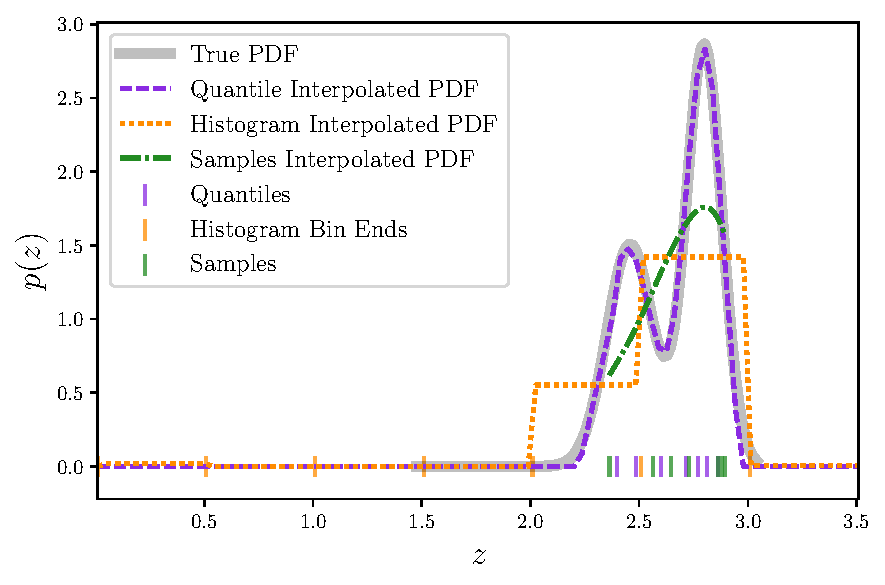
\includegraphics[width=\columnwidth]{figures/demo_pz.pdf}
    \caption{\qp\ approximation of a continuous 1-dimensional PDF (solid black 
line) using the step function (orange dotted line), samples (green dash-dotted 
line), and quantile formats (purple dashed line) with the same number of stored 
parameters ($N_{f}=7$ in this case).
    \label{fig:qp}}
  \end{center}
\end{figure}
For each format, we address the following questions:
\begin{itemize}
  \item When/where has this format appeared in the literature as a published 
catalog format, native \pz\ code output format, and science application input 
format?
  \item What exactly is stored under this format, per galaxy (the parameters) 
and per catalog (the metaparameters)?
  \item Beyond fidelity to the original \pz, what are the a priori strengths 
and weaknesses of this format?
\end{itemize}

\subsubsection{Regular Binning}
\label{sec:bins}

By far the most popular format for approximating and storing \pz s is that of a 
piecewise constant step function, also called a histogram binning 
\citep{carrasco_kind_somz:_2014, sadeh_annz2:_2016, cavuoti_metaphor:_2017}.
It is the only format that has been used for public release of \pz\ catalogs 
\citep{tanaka_photometric_2017, sheldon_photometric_2012}; it is unclear 
whether this is a consequence or cause of the fact that it is the most common 
format for using \pz s in cosmological inference, as tomographic binning is a 
universal step between the \pz\ catalog and calculation of any two-point 
correlation function.

The metaparameters of the binned parametrization are the ordered list of 
redshifts $\vec{C} = (z_{1}, z_{2}, \dots, z_{N_{f}}, z_{N_{f}+1})$ serving as 
bin endpoints shared by all galaxies in the catalog, each adjacent pair of 
which is associated with a parameter $c_{i}=\int_{C_{i}}^{C_{i+1}}\ p(z)dz$.
The \qp\ histogram format assumes $p(z)=0$ when $z<C_{1}$ or $z>C_{N_{f}+1}$, 
leading to the normalization condition $\sum_{i} c_{i}(C_{i+1}-C_{i})) = 1$.
\footnote{Note that this is not generally equivalent to the erroneous 
normalization condition $\sum_{i} c_{i} = 1$ commonly enforced in public 
catalogs.}
The histogram format function $\mathcal{F}^{h}$ is the sum of a set of $N_{f}$ 
step functions, making the reconstructed estimator of the \pz
\begin{align}
  \label{eq:binned}
  \hat{p}^{h}(z) &= \sum_{i}^{N_{f}}\ c_{i} 
\left\{\begin{tabular}{cc}$1$&$C_{i}<z<C_{i+1}$\\
0&$z < C_{i}$\ or\ $z > C_{i+1}$\end{tabular}\right\},
\end{align}
where the step functions may be considered their own interpolators.
Here we only consider a regular binning, with $C_{i+1}=C_{i}+\delta_{f}$ for a 
constant $\delta_{f}=(C_{N_{f}+1}-C_{1})/N_{f}$, as this is the only type of 
binning that has been used in the literature, but this condition is not 
required by \qp.

The regular histogram format may be considered wasteful in terms of data 
storage; a \pz\ with a very compact (broad) probability distribution may have 
many parameters taking the same value $c_{i}\approx0$ 
($c_{i}\approx(C_{N_{f}+1}-C_{1})\delta^{-1}$) that are redundant in storage.

\subsubsection{Random Samples}
\label{sec:samples}

Samples are the native output format of many machine learning algorithms due to 
the discrete nature of training sets \citep{de_vicente_dnf_2016}.
Such approaches typically produce large numbers of samples, far more than can 
realistically be stored by any survey, so a subsample is commonly stored.
Samples are easy to use in standard science applications developed for redshift 
point estimates, so they have an established presence in the literature 
\citep{dark_energy_survey_collaboration_redshift_2016}.

The parameters of the samples format are the $N_{f}$ samples $\vec{c}=(z_{1}, 
z_{2}, \dots, z_{N_{f}-1}, z_{N_{f}})$, where $C=N_{f}$ is an implicit 
metaparameter.
Though it is possible to construct a catalog where $C$ is not uniform over the 
catalog, but is instead somehow optimized for each galaxy, we leave its 
investigation to future work, as it has not yet appeared in the literature.
The format function $\mathcal{F}^{s}$ that turns samples into a representation 
of the \pz\ is simply the interpolator $F$; in the tests presented here, we use 
the Gaussian kernel density estimate (KDE) of 
\texttt{scipy.stats.gaussian\_kde} with the smoothing bandwidth $C'$ as a 
metaparameter.  The samples representation is then
\begin{align}
  \label{eq:sampled}
  \hat{p}^{s}(z) &= F_{C'}(z; \vec{c}).
\end{align}

Though samples are an obvious choice for \pz s with narrow features of high 
amplitude, we expect that using a small number of samples from a broad \pz\ may 
increase the variance of any ensemble metrics, as the sampling introduces 
additional shot noise.
The researcher must also choose an interpolation method to reconstruct a \pz\ 
from samples.

\subsubsection{Regular Quantiles}
\label{sec:quantiles}

One parametrization that has not previously been investigated in the context of 
photometric redshifts is that of quantiles, which are defined in terms of the 
cumulative distribution function (CDF).
The quantile format for expressing a PDF, however, has appeared in the 
astronomy literature \citep{sun_star_2015, pizzocaro_results_2016, 
laycock_x-ray_2017}.

Under the quantile format, a \pz\ catalog shares $N_{f}$ ordered CDFs 
$\vec{C}=(q_{1}, q_{2}, \dots, q_{N_{f}-1}, q_{N_{f}})$.
Each galaxy's catalog entry is the vector of redshifts $\vec{c}=(z_{1}, z_{2}, 
\dots, z_{N_{f}-1}, z_{N_{f}})$ satisfying $CDF(c_{i})=C_{i}$, so the quantile 
format function $\mathcal{F}_{q}$ is the derivative of an interpolation of the 
inverse CDF $CDF^{-1}(C_{i})=c_{i}$ under the interpolation scheme $F$.
In this study, we test regular quantiles $C_{i}\equiv i(N_{f}+1)^{-1}$ using a 
\texttt{scipy.interpolate} spline interpolation scheme in the quantile range 
and linear extrapolation outside it.
The format function is then the convolution $\mathcal{F}^{q}=F(CDF^{-1})$, 
making the quantile representation
\begin{align}
  \label{eq:quantiles}
  \hat{p}^{q}(z) &= F\left(z; \vec{c}, 
\frac{\Delta\vec{C}}{\Delta\vec{c}}\right).
\end{align}


A quantiles parametrization (the namesake of the \texttt{qp} code) is expected 
to be an efficient approximation for \pz s because it allocates storage evenly 
in the space of probability density.
In contrast, the histogram format stores data evenly spaced in redshift, and 
the samples format stores data randomly in probability density.
As with the samples representation, an interpolation function must be chosen 
for reconstructing the \pz\ from the stored parameters.
Depending on the native \pz\ output format, converting to the quantile format 
may require $N_{f}$ numerical optimizations to find the quantiles.
We accelerate these optimizations by initializing at rough, approximate 
quantiles based on CDF evaluations on a grid.





\subsection{Comparison Metrics}
\label{sec:metric}

In this work, our aim is to probe how closely \pz s reconstructed from limited 
set of stored parameters approximate their original, high-resolution 
representation.
This is done without reference to a galaxy's true redshift; there is, in fact, 
no notion of a true redshift in our analysis.
(For a demonstration of how one might approach the distinct problem of 
evaluating the accuracy of a \pz\ relative to a true redshift, see Schmidt, et 
al.\ in preparation.)

We consider as a metric the loss of information, measured in nats (base $e$ 
bits), incurred when using an approximation of the PDF $\hat{P}(z)$ instead of 
the best possible representation of the  PDF $P(z)$, given by the 
Kullback-Leibler divergence (KLD), which is defined as
\begin{align}
  \label{eq:kld}
  \mathrm{KLD}[\hat{P}(z) | P(z)] &= \int_{-\infty}^{\infty}\ P(z)\ 
\log\left[\frac{P(z)}{\hat{P}(z)}\right]\ dz,
\end{align}
where $\log$ is the natural logarithm throughout this paper unless indicated 
otherwise.
Because there is in general no closed-form expression for the KLD, we calculate 
the discrete KLD
\begin{align}
  \label{eq:kld_approx}
  \mathrm{KLD}[\hat{P}(z) | P(z)] &\approx 
\delta_{ff}\sum_{z=z_{1}}^{z_{N_{ff}}}\ P(z)\ 
\log\left[\frac{P(z)}{\hat{P}(z)}\right]
\end{align}
using evaluations of the PDF under each format on a very fine, regular grid 
$(z_{1}, z_{2}, \dots, z_{N_{ff}-1}, z_{N_{ff}})$ with resolution 
$\delta_{ff}\ll\delta_{f}$.

The most important feature of the KLD is its asymmetry; it is not a distance, 
like the root mean square error, that is the same from $P(z)$ to $P'(z)$ as it 
is from $P'(z)$ to $P(z)$ but a \textit{divergence} in the information lost 
when using $P'(z)$ to approximate $P(z)$, or, in other words, the information 
gain in going from $P'(z)$ to $P(z)$.
The KLD requires that both functions $P(z)$ and $P'(z)$ be probability 
distributions (always positive semidefinite and integrating to unity); this may 
need to be explicitly enforced for some approximation formats.
The KLD is always positive, and a smaller value indicates better agreement 
between the approximation and the truth.
We review the properties of the KLD and provide some intuition for it in the 
Appendix.

Additionally, we employ the percent error
\begin{align}
  \label{eq:percent_error}
  \mathrm{P.E.}[M_{m}[\hat{P}(z)] | M_{m}[P(z)]] &= \frac{M_{m}[P(z)] - 
M_{m}[\hat{P}(z)]}{M_{m}[P(z)]}\times100\%
\end{align}
of the moments
\begin{align}
  \label{eq:moment}
  M_{m}[P(z)] &= \int_{-\infty}^{\infty} z^{m}\ P(z)\ dz\ \approx\  
\delta_{ff}\sum_{z=z_{1}}^{z_{N_{ff}}}\ z^{m}\ P(z)
\end{align}
of a PDF.
We note that $M_{0}[(P(z)]=1$ for all properly normalized probability 
distributions, $M_{1}[(P(z)]=\bar{z}$ is the mean, $M_{2}[(P(z)]$ is the 
variance, and $M_{3}[(P(z)]$ is the kurtosis.
Though the first few moments are not in general sufficient to characterize a 
highly structured probability distribution, they are included in this analysis 
because they can prove useful in setting ballpark estimates of the influence of 
different systematics in various science cases.

\subsubsection{Individual \pz s}
\label{sec:individual_metric}

Some science applications rely on the recovery of individual galaxy \pz s that, 
for example, may be used as the basis for targeting spectroscopic follow up.
For this purpose, we calculate the KLD of each individual \pz\ in our catalogs 
and then characterize the distribution of KLD values (which is itself a PDF) by 
its $m=1,\ 2,\ 3$ moments.
We also calculate the percent error on the $m=1,\ 2,\ 3$ moments of each \pz\ 
under all parametrizations and use the median and interquartile range of the 
moment percent error distribution $p(M_{m}[\hat{p}_{i}(z)])$ of the ensemble as 
another metric of the fidelity of individual \pz\ parametrizations.
We use these aggregate statistics to observe how the approximate individual \pz 
s for each dataset vary with the choice of parametrization.

\subsubsection{Stacked $\hat{n}(z)$ estimator}
\label{sec:stacked_metric}

In addition to considering how the choice of storage parametrization affects 
the recovery of individual \pz s, we also demonstrate how one might use 
\texttt{qp} to choose the best parametrization for a particular science case.
We encourage users to develop a metric around their own \pz\ use cases, as the 
optimal parametrization may not be shared among all science applications of \pz 
s.

In cosmology, \pz s have thus far been used almost exclusively to estimate the 
redshift distribution function $n(z)$ necessary for calculating the correlation 
functions used by many cosmological probes.
The most common way to estimate the redshift distribution function for a sample 
of $N_{g}$ galaxies is to sum the \pz s according to
\begin{align}
  \label{eq:nz}
  \hat{n}(z) &\equiv \frac{1}{N_{g}}\ \sum_{k=1}^{N_{g}}\ \hat{p}_{k}(z),
\end{align}
a procedure known as stacking.
We refer to $\hat{n}(z)$ as the stacked estimator of the redshift distribution 
and denote the stacked estimator derived from the original input \pz s as 
$\hat{n}'(z)'$.
While we do not recommend this approach to estimating the redshift distribution 
(see Malz and Hogg, et al.\ (in preparation) for an alternative method), we use 
it here on the assumption that any metric calculated for a more principled 
estimator will have similar behavior with respect to the parametrization of the 
\pz\ catalog.
This assumption may be tested in future work.

As the stacked estimator is normalized so that it, too, is a PDF (though in the 
literature it is often subject to the fallacy conflating a sum and an integral, 
first mentioned in Sec. \ref{sec:bins}), the KLD \textit{from} the stacked 
estimator of a catalog of evaluations of reconstructed \pz s \textit{to} the 
stacked estimator of a catalog of evaluations of the original, high-resolution 
\pz s serves as a metric for a specific science use case of \pz s.
Because the accuracy of lower-order moments of the redshift distribution 
function dominates the weak lensing error budget, we also compare the percent 
error on the $m=1,\ 2,\ 3$ moments of $\hat{n}(z)$.
However, this information may be less relevant due to the broad range of 
redshifts and small number of galaxies considered in each instantiation.
Furthermore, we note that the domination of the first few moments of 
$\hat{n}(z)$ may not always hold true as the methodology of \pz\ usage in 
cosmology evolves.


\section{Photo-z Test Data}
\label{sec:data}

With the expectation that the optimal parametrization for approximating \pz s 
may differ according to the properties of the original photometric data, we 
demonstrate a procedure for vetting \pz\ parametrizations on a pair of mock 
datasets, each intended to be realistic projections of subsets of the 
anticipated LSST \pz s.
All \pz s were fit using the publicly available Bayesian Photometric Redshift 
(BPZ) code \citep{benitez_bayesian_2000}, which employs spectral energy 
distribution (SED) fitting to a template library.
The choice of \pz\ estimation method, however, is not relevant to this study; 
so long as the mock \pz s are \textit{realistically complex}, meaning they take 
shapes similar to those we expect to see in \pz s from real datasets with 
similar photometric properties, it does not matter whether the \pz s produced 
by BPZ are accurate redshift posteriors.
We seek only to optimize the fidelity of the stored \pz\ relative to the \pz\ 
output by a representative \pz\ fitting code.
\citep[See][Schmidt, et al.\ in preparation for other work comparing the 
accuracy of \pz s produced by different methods.]{tanaka_photometric_2017}
As BPZ is a widely used and well established method, we assume that the \pz s 
produced by it are of representative complexity.
The default format of BPZ is a $N_{ff}>200$ gridded parametrization with 
resolution exceeding the available storage for any planned survey.
Because we believe that each galaxy has an underlying redshift interim 
posterior probability distribution that is a continuous function, to which the 
output of BPZ is itself a high-resolution approximation in the form of 
evaluations on a grid, we fit each gridded \pz\ with a Gaussian mixture model 
that we designate as the reference representation for our accuracy tests.

\begin{figure*}
  \begin{center}
    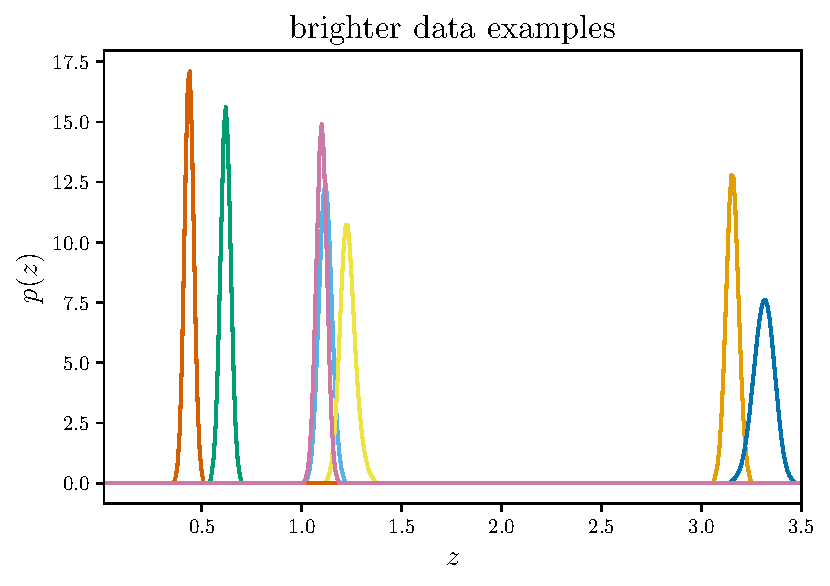
\includegraphics[width=\columnwidth]{figures/graham_pzs.pdf}
    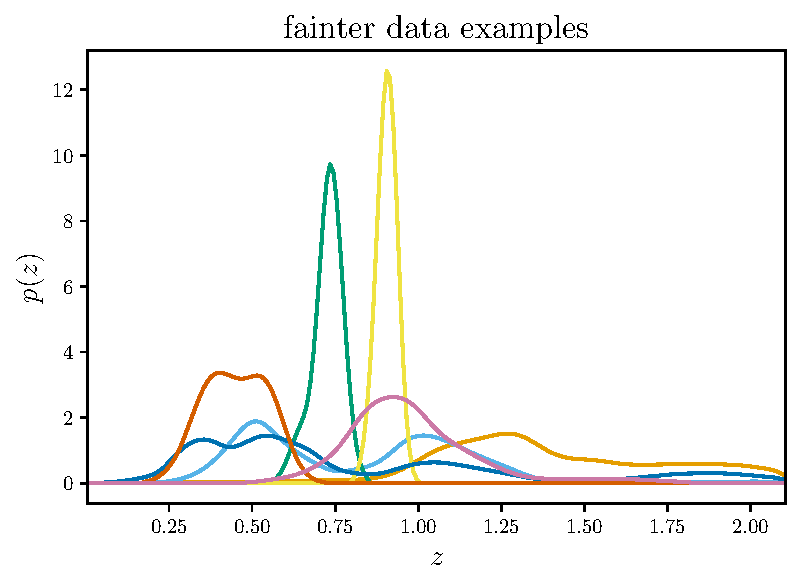
\includegraphics[width=\columnwidth]{figures/schmidt_pzs.pdf}
    \caption{
    Example \pz s from the two mock LSST datasets.
    Left: The \mgdata mock photometry yields largely narrow, unimodal \pz s.
    Right: The \ssdata mock photometry contains a higher proportion of broad 
and/or multimodal \pz s.
    \label{fig:example_pzs}}
  \end{center}
\end{figure*}

\subsection{\Mgdata data mock catalog}
\label{sec:graham}

Our first dataset is an $N_{g}=100,000$ object subset of the simulated galaxy 
catalog used for LSST photometric redshift experiments by 
\citet{graham_photometric_2017}.
The data builds on the Millennium simulation \citep{springel_simulations_2005}, 
and in particular the LC DEEP catalog based on the galaxy formation models of 
\citet{gonzalez-perez_how_2014}, and was created using the lightcone 
construction techniques described by \citet{merson_lightcone_2013}.
We limit the sample to galaxies with a catalog $i$-band magnitude of $i<25$ and 
true redshifts $z<3.5$.
As in Graham, et al. (in preparation), we simulate observed apparent magnitudes 
from the true catalog magnitudes by adding a normal random scatter with a 
standard deviation equal to the predicted magnitude error for each galaxy (from 
Section 3.2.1. of \citet{ivezic_lsst:_2008}, using the software of 
\citet{connolly_end--end_2014}, assuming a mean airmass of 1.2 and a 10-year 
accumulation of 56, 80, 184, 184, 160, and 160 visits in filters $ugrizy$, 
respectively).
We also ignore any magnitudes fainter than the predicted 10-year limiting 
magnitudes in each filter, $u<26.1$, $g<27.4$, $r<27.5$, $z<26.1$, and 
$y<24.9$, as a realistic simulation of non-detections.

The \pz\ estimates for this simulated catalog use the CFHTLS set of spectra 
\citep{ilbert_accurate_2006} as BPZ templates and the default parameter 
settings for BPZ, except that we impose a maximum photometric redshift of 3.5 
and allow BPZ to use the $i$-band as a magnitude prior during the photo-$z$ fit.
The \pz s from BPZ are in the form of $N_{ff} = 351$ evaluations of the 
probability density on a regular grid of redshifts $0.01 < z < 3.51$, a 
subsample of which are plotted in the left panel of 
Figure~\ref{fig:example_pzs}.

As the figure shows, the \pz s from this dataset tend to be unimodal and 
sharply peaked, as if coming from brighter photometric data due to the 
conservative cuts in photometric magnitudes of this dataset.
We produce reference \pz s for the analysis by fitting a three-component 
Gaussian mixture model to each \pz\ in the catalog, where the number of 
components was chosen to be the $99^{\mathrm{th}}$ percentile of the modality 
distribution of the gridded \pz s.
We then calculate the three approximations to each \pz\ and evaluate their 
accuracy using the metrics described above.

\subsection{\Ssdata data mock catalog}
\label{sec:schmidt}

Our second dataset is an independent simulation of the expected LSST galaxy 
sample.
Here, we use the Buzzard-highres-v1.0 mock galaxy catalog of deRose, et al.\ 
(in preparation) of galaxies with SEDs drawn from an empirical library of 
$\sim500,000$ SEDs from the Sloan Digital Sky Survey (SDSS).
Given an SED, redshift, and absolute $r$-band magnitude for each galaxy, we 
compute the expected apparent magnitudes and magnitude errors in the six 
broadband LSST filters ($ugrizy$), assuming the full 10-year depth of the 
survey using the simple model of \citet{ivezic_lsst:_2008}.
The catalog contains $N_{g}\approx100,000$ galaxies $z<2.105$ to a depth of 
$i<26.9$, 1.5 magnitudes deeper than the expected LSST Gold sample of galaxies 
that will have $S/N\gtrsim30$ in multiple bands.

In implementing BPZ, we createed a custom Bayesian prior using a subset of the 
Buzzard-highres-v1.0 catalog and a spanning template set via a simple k-means 
clustering algorithm based on $100$ of the SDSS SEDs used in creating the 
Buzzard catalog.
BPZ produces \pz s in the format of probability density evaluations on a 
regular grid of $N_{ff}=211$ redshifts $0.005\leq z\leq2.105$, a subsample of 
which are plotted in the right panel of Figure~\ref{fig:example_pzs}.

Even with six filters spanning the optical, there are known degeneracies 
(e.~g.~the Lyman/Balmer break degeneracy) that lead us to expect the presence 
of multimodal \pz s.
The exceptional depth of the dataset also leads us to expect the presence of 
broad \pz s.
We produced reference \pz s for the analysis by fitting a five-component 
Gaussian mixture model to each gridded \pz\ in the catalog, where the number of 
components was chosen to equal the $99^{\mathrm{th}}$ percentile of the 
modality distribution of the gridded \pz s.
We then calculated the three different approximations to each \pz, and 
evaluated their accuracy using the metrics described above.


\section{Results \& Discussion}
\label{sec:results}

We calculate the metrics of Section~\ref{sec:metric} on 10 random 
instantiations of catalogs of $N_{g}=100$ galaxies drawn randomly from each of 
the datasets discussed in Section~\ref{sec:data} and with each of $N_{f}=3,\ 
10,\ 30,\ 100$ stored parameters.
We then illustrate how our results could be used to choose an appropriate 
parametrization for each dataset given constraints on the distribution of KLDs 
or moment percent errors of individual \pz s, the KLD or moment percent error 
of $\hat{n}(z)$, or the available storage capacity.


\subsection{Individual \pz s}
\label{sec:individual_results}

We compare our three parametrizations on the basis of the distributions of the 
KLD calculated for every \pz\ in the dataset.
An example of an individual \pz\ KLD distribution for the \mgdata dataset with 
$N_{f}=10$ is shown in Figure~\ref{fig:individual}.
\begin{figure}
  \begin{center}
    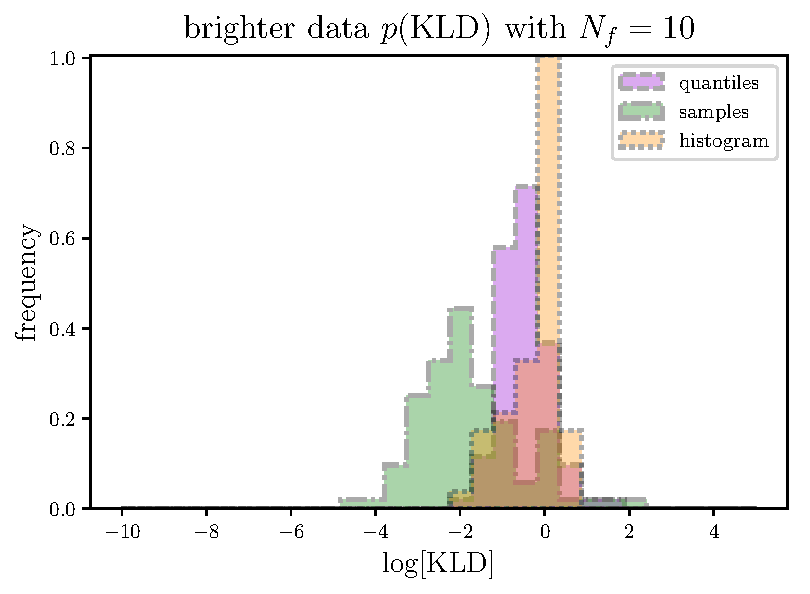
\includegraphics[width=\columnwidth]{figures/individual_kld.pdf}
    \caption{The distribution of log-KLD values for $N_{g}=100$ \pz s from the 
\mgdata dataset with $N_{f}=10$ over the quantiles (purple with dashed border), 
samples (green with dash-dotted border), and histogram (orange with dotted 
border) formats.
    In this instantiation, the samples format has a lower median KLD than the 
quantiles format, which has a lower median KLD than the piecewise constant 
format.
    Note that the distributions are over log-KLD, so the ordering of the 
formats by the breadth of the log-KLD distribution is the same as the order by 
the median.
    \label{fig:individual}}
  \end{center}
\end{figure}

To distill what is observed in the ten instantiations of plots like 
Figure~\ref{fig:individual} for both datasets and all parametrizations, we 
compare the moments of the distributions of metric values for the distribution 
of the KLDs of individual \pz s under each parametrization, summarized in 
Figure~\ref{fig:kld_moments}.
While it is obvious that one would like the mean (first moment) of the KLD 
distribution to be low, interpretation of higher-order moments is less clear.
In a science application that is robust to \pz\ outliers, a parametrization 
with a high variance (second moment) may be acceptable, whereas in another 
science application that simply requires well-characterized errors could 
tolerate a higher mean in exchange for a lower variance.
To meaningfully interpret the KLDs of individual \pz s, it will be necessary 
for those using \pz s in their science to calculate the requirements on the 
acceptable degree of information loss.
\begin{figure*}
  \begin{center}
    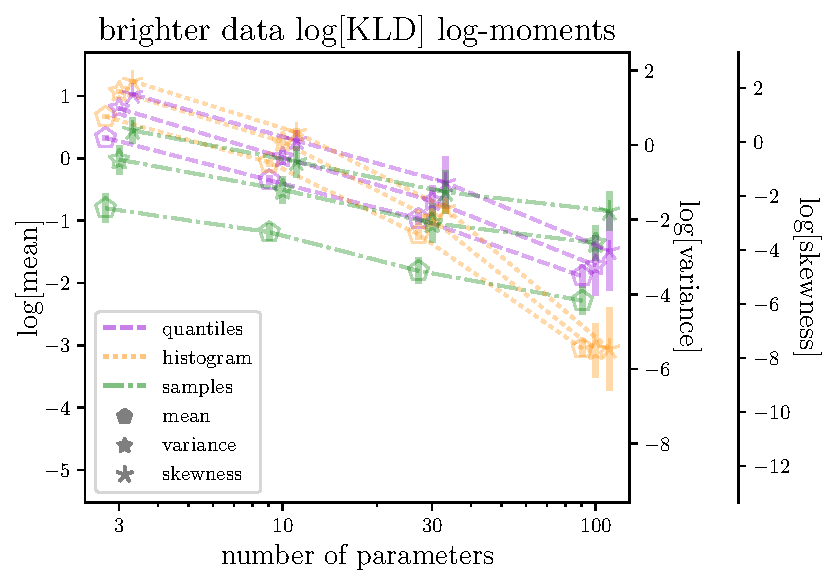
\includegraphics[width=\columnwidth]{graham_pz_kld.pdf}
    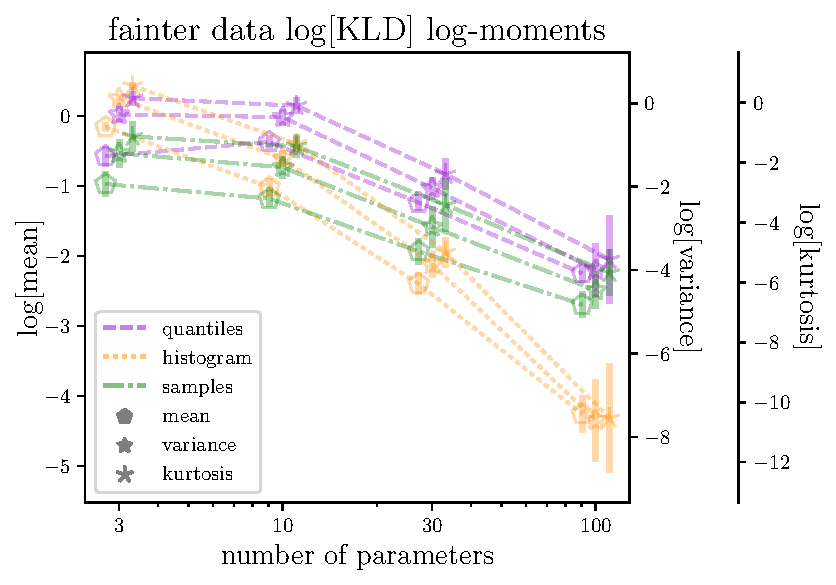
\includegraphics[width=\columnwidth]{schmidt_pz_kld.pdf}
    \caption{
    The means of the mean ($\bigstar$), variance ($+$), and kurtosis ($\times$) 
of the log-KLD distributions for each dataset as a function of the number 
$N_{f}$ of stored parameters for the quantile (dashed purple line), samples 
(dash-dotted green line), and histogram (dotted orange line) formats with 
$1\sigma$ Gaussian error bars based on 10 instantiations of 100 galaxies, which 
are offset about $N_{f}$ to improve readability.
    Left panel: The distribution of individual \pz\ KLD values of the \mgdata 
mock catalog is most well-behaved when they are stored as samples, except at 
large $N_{f}$.
    Right panel: The \ssdata mock catalog achieves equivalence of the formats 
in the moments of the log-KLD distributions at a much lower $N_{f}$, ultimately 
showing the histogram format is most well-behaved at all but the smallest 
$N_{f}$.
    \label{fig:kld_moments}}
  \end{center}
\end{figure*}

Figure~\ref{fig:kld_moments} is rich in information.
For both datasets, the behavior of the first three log-moments of the log-KLD 
distribution is highly correlated for a given format and number of parameters.
The \mgdata dataset has higher log-KLD log-moments than the \ssdata dataset at 
all $N_{f}$ and across all formats, meaning information loss is enhanced for 
more strongly featured data; this observation is not surprising because the 
narrow, unimodal \pz s of the \mgdata dataset have long tails of very low 
probability that are emphasized by the KLD.
The \ssdata dataset shows almost no change in the log-KLD log-moments between 
$N_{f}=3$ and $N_{f}=10$ parameters, but both datasets otherwise exhibit a 
steady decrease in all moments for the quantile and samples formats as $N_{f}$ 
increases.
The log-KLD log-moments are higher for quantiles than for samples for both 
datasets, except at $N_{f}=100$ for the \mgdata dataset.
The histogram format's log-KLD log-moments are higher than for other formats at 
low $N_{f}$ and steadily decrease in a manner similar to the other formats, 
except at the highest $N_{f}$ values where the histogram format's log-KLD 
log-moments decrease much more quickly.
The error bars on the log-KLD log-moments increase at high $N_{f}$ for all 
formats on both datasets beyond what one would expect simply based on the log 
scaling.

We also examine the percent error on the first three moments of the \pz s under 
each approximation, using the base-10 log for interpretability.
Because the distribution of moment percent errors is highly non-Gaussian due to 
a small number ($<1\%$) of truly extreme outliers for both datasets, across all 
$N_{f}$ and all formats, we substitute the interquartile range for traditional 
$1\sigma$ Gaussian error bars.
\begin{figure*}
  \begin{center}
    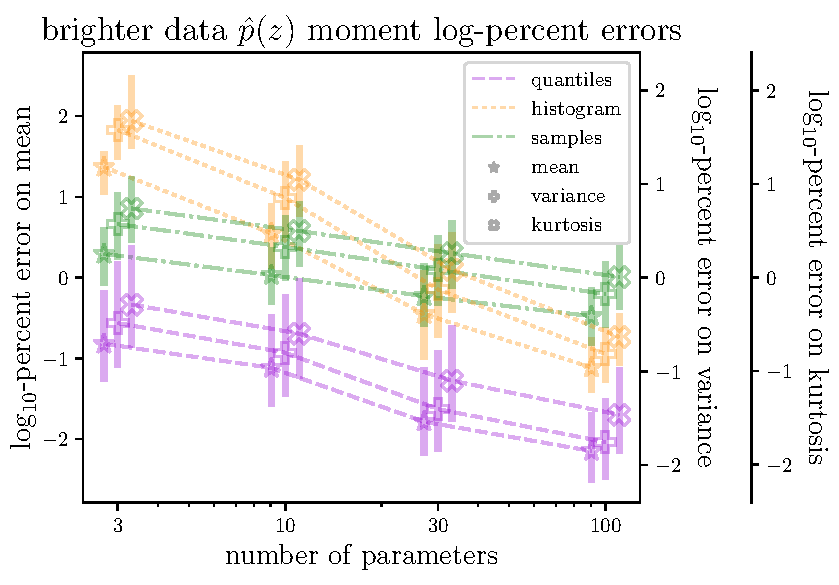
\includegraphics[width=\columnwidth]{graham_pz_err.pdf}
    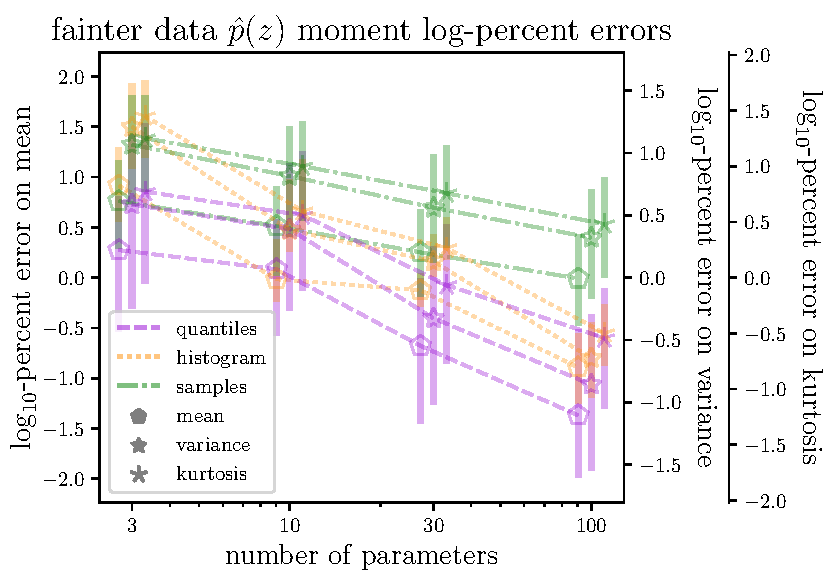
\includegraphics[width=\columnwidth]{schmidt_pz_err.pdf}
    \caption{
   The median $\log_{10}$-percent errors on the mean ($\bigstar$), variance 
($+$), and kurtosis ($\times$) of the \pz s for each dataset as a function of 
the number $N_{f}$ of stored parameters per \pz\ for the quantile (dashed 
purple line), samples (dash-dotted green line), and histogram (dotted orange 
line) formats with interquartile range error bars based on 10 instantiations of 
100 galaxies, where the $\log_{10}$-percent errors and their interquartile 
ranges are offset around $N_{f}$ to improve readability.
   Left panel: The \mgdata \pz\ ensemble's moment percent errors are minimized 
by the quantile format at all $N_{f}$.
   Right panel: The \ssdata \pz\ ensemble's moment percent errors are high for 
all formats at low $N_{f}$ but distinct at high $N_{f}$, with the quantile 
format ultimately outperforming the samples and histogram formats.
    \label{fig:pz_moment_errs}}
  \end{center}
\end{figure*}

Though the $\log_{10}$-percent error of the moments of individual \pz s also 
exhibits significant correlation between the moments for a given 
parametrization, the behavior is otherwise markedly different from that of the 
log-moments of the \pz\ ensemble's log-KLD distribution.
The percent errors on the moments of the approximate \pz s are overall lower in 
the \mgdata dataset than the \ssdata dataset over the same range of number of 
stored parameters; this is expected because there is simply less information to 
capture in the \mgdata dataset.

For the \mgdata dataset, the quantile format enables sub-percent errors in \pz\ 
moments at the lowest $N_{f}$, a level that cannot be achieved by the histogram 
format until $N_{f}=100$ parameters are stored and by samples at fewer than 
$N_{f}=100$ stored parameters.
Furthermore, for the \mgdata dataset, the quantile format minimizes the percent 
error at all $N_{f}$, whereas the samples format is better than the histogram 
format at low $N_{f}$ but the histogram format is better than the samples 
format at high $N_{f}$.
Again, this behavior is expected of the narrow, unimodal \pz s of the \mgdata 
dataset because large histogram bins are ineffective at capturing small-scale 
structure and including more samples does not significantly improve 
preservation of such features.

Though the \ssdata dataset has an ordering of the percent error on the moments 
at $N_{f}=3$ that is similar to that of the \mgdata dataset, all formats, not 
just the histogram format, have shockingly high errors, meaning it is highly 
inappropriate to use so few parameters for such a faint dataset even if it may 
be acceptable for a brighter one.
In the \ssdata dataset, the inclusion of $N_{f}=30$ parameters decreases the 
percent error of the moments of the histogram format more significantly than 
the quantile or samples formats, to the point that the histogram and quantiles 
formats are comparable.
At higher $N_{f}$ in the \ssdata dataset, the quantile and histogram formats 
continue to improve faster than the samples format, with the percent errors on 
the \pz\ moments being consistently lower for the quantile format than for the 
histogram format.
With the broad, multimodal \pz s of the \ssdata dataset, sub-percent accuracy 
in the moments can only be achieved with $N_{f}\geq30$ with the quantile format 
and $N_{f}=100$ with the histogram format.

\subsection{Stacked $\hat{n}(z)$ estimator}
\label{sec:stacked_results}

Figure~\ref{fig:stacked} shows an example of $\hat{n}(z)$ of \pz s 
reconstructed from just $N_{f}=10$ parameters under each of our three 
approximation formats, evaluated on the same fine grid as the input \pz s.
The strong features in the curve are due to the very small sample size of $100$ 
galaxies.
As expected, the stacked histogram is quite coarse because of the step function 
interpolation, while the stacked estimator of the redshift distribution based 
on \pz\ representations that are interpolations of stored samples and quantiles 
are much closer to the stacked estimator of the original, high-resolution \pz s.
The KLD for each format is also included in the plot; in this instance, the KLD 
is lowest for the quantile format and highest for the histogram format.

\begin{figure}
  \begin{center}
    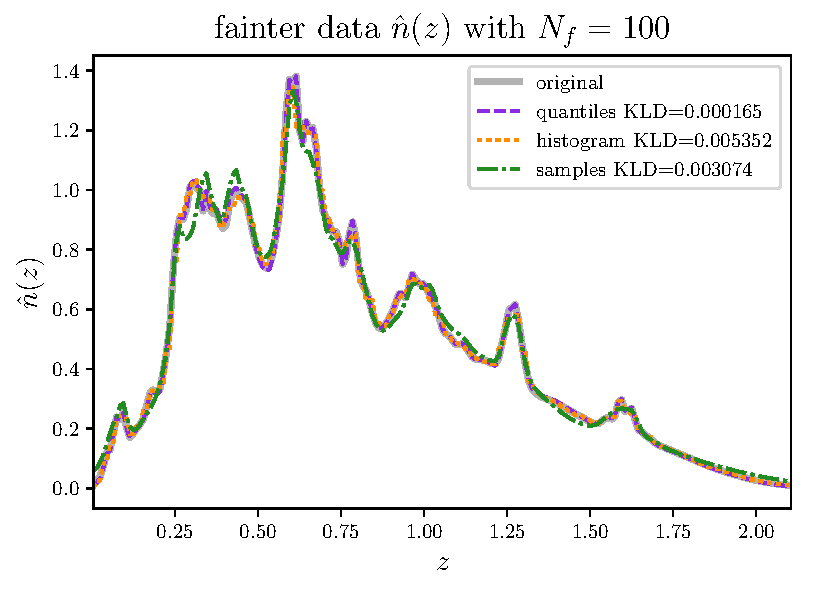
\includegraphics[width=\columnwidth]{figures/stacked.pdf}
    \caption{An example of the stacked estimator of the redshift distribution, 
for a subsample of $N_{g}=100$ galaxies drawn from the \ssdata data mock 
catalog and with just $N_{f}=10$ parameters used for each \pz; the small-scale 
features are due to the small number of galaxies in the sample.
    The most striking characteristic of $\hat{n}(z)$ with a relatively small 
number of parameters on a small number of galaxies is the coarseness of the 
histogram format (orange dotted line) relative to the quantile format (purple 
dashed line) and samples format (green dash-dotted line), both of which are 
fairly close to $\hat{n}(z)$ derived from evaluating the original, 
high-resolution \pz s (thick gray line).
    \label{fig:stacked}}
  \end{center}
\end{figure}

Again, due to the variation between $N_{g}=100$ galaxy subsamples, we repeat 
the procedure that produced Figure~\ref{fig:stacked} 10 times to generate a 
distribution over the KLD of the stacked estimator of the redshift distribution 
for each format for each dataset.
The $\hat{n}(z)$ KLD values for each parametrization on both mock datasets are 
collected and plotted in Figure~\ref{fig:kld}, with error regions based on the 
variance between the 10 instantiations.
\begin{figure*}
  \begin{center}
    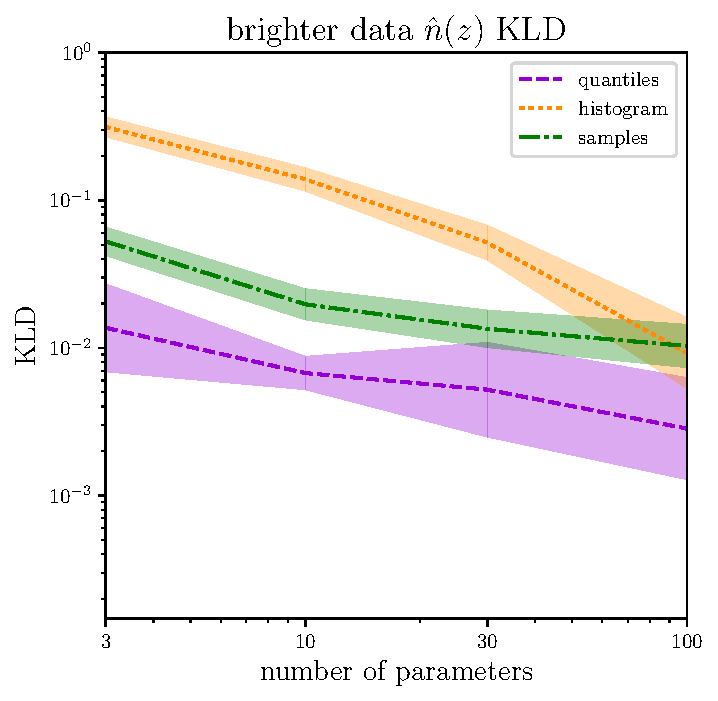
\includegraphics[width=\columnwidth]{figures/graham_nz_kld.pdf}    
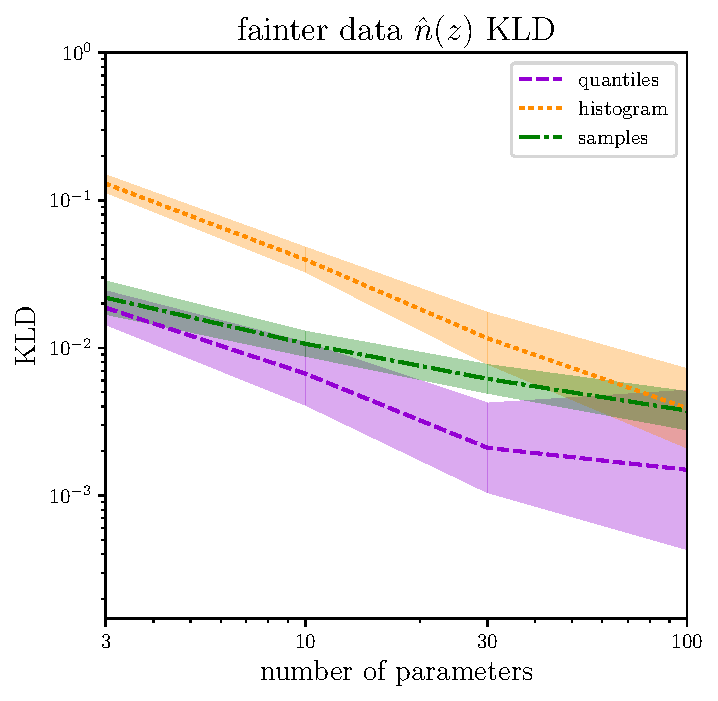
\includegraphics[width=\columnwidth]{figures/schmidt_nz_kld.pdf}
    \caption{KLD between $\hat{n}(z)$ derived from approximate pz\ 
representations and  $\hat{n}(z)$ derived from the original, high-resolution 
\pz s as a function of number $N_{f}$ of stored parameters, for the quantiles 
(purple dashed line), samples (green dash-dotted line), and histogram (orange 
dotted line) formats, with shaded regions indicating the $1\sigma$ Gaussian 
errors derived from 10 subsamples of 100 galaxies and lines indicating the mean 
of the distribution.
    Left panel: The \mgdata \pz\ catalog's KLD of $\hat{n}(z)$ is minimized by 
the quantile format at all $N_{f}$ but with a larger scatter than other formats.
    Right panel: The \ssdata \pz\ catalog's KLD of $\hat{n}(z)$ is minimized by 
the quantile format at all $N_{f}$, though the samples format also has a 
comparably low KLD with lower scatter.
    \label{fig:kld}}
  \end{center}
\end{figure*}
Figure~\ref{fig:kld} shows that the two datasets clearly share some features:
\begin{enumerate}
\item As expected, the KLD drops as the number of stored parameters increases, 
for all formats.
\item The quantile format minimizes the KLD at all numbers of stored parameters 
considered but has a larger variance between instantiations than the other 
formats.
\item The histogram format leads to substantial loss of information relative to 
the other formats except at large numbers of stored parameters where it is 
comparable with the samples format.
\end{enumerate}
However, there are also ways in which the behavior of the KLD on $\hat{n}$ 
differs due to the data quality's significant impact on the behavior of this 
metric:
\begin{enumerate}
\item The \ssdata dataset enables the achievement of lower KLD values than the 
\mgdata dataset for all formats at all values of $N_{f}$ considered, likely a 
consequence of the strong features present in $\hat{n}(z)$ for the \mgdata 
dataset in our subsamples of 100 galaxies.
\item The rate at which the KLD of $\hat{n}(z)$ improves with increasing $N_{f} 
$ is overall slower for the \mgdata dataset than for the \ssdata dataset; in 
other words, saving more parameters has a greater marginal benefit for a 
\ssdata dataset than for a \mgdata dataset.
\item The $\hat{n}(z)$ KLD for the samples format is not substantially higher 
than for the quantile format for the \ssdata dataset but is for the \mgdata 
dataset, which may reflect the subjectivity of the reconstruction scheme used 
for those two formats.
\end{enumerate}

We also address the relative, marginal, and absolute performance and 
consistency thereof of the KLD on $\hat{n}$ for each parametrization as a 
function of format and $N_{f}$ for each dataset.
To guide this process, we interpret Figure~\ref{fig:kld} in the context of 
constraints on the acceptable degree of information loss imposed by the science 
requirements and constraints on storage allocation imposed by the survey.

A constraint on the acceptable loss of information due to compression and 
reconstruction of \pz s corresponds to a horizontal line at some 
$\mathrm{KLD}_{\mathrm{lim}}$ in Figure~\ref{fig:kld}; the best parametrization 
would correspond to the format that achieves $\mathrm{KLD}_{\mathrm{lim}}$ at 
the lowest $N_{f}$.
For example, if $\mathrm{KLD}_{\mathrm{lim}}=10^{-2}$ nats, the quantile 
parametrization with $N_{f}=3$ would be optimal due to the slow marginal 
improvement of the $\hat{n}(z)$ KLD for the \mgdata dataset for the quantiles 
and samples format and the high values of the KLD for the histogram format.
If the \ssdata dataset were subject to the same constraint, the quantile 
parametrization with $N_{f}=10$ achieves the limiting KLD at the lowest 
$N_{f}$, but the samples format achieves the same limit with a smaller scatter 
at $N_{f}=30$ so might be considered more reliable.

A constraint on storage resources corresponds to a vertical line at a given 
$N_{f, \mathrm{lim}}$ in Fig. \ref{fig:kld}; the best format would be the one 
that achieves the lowest KLD at $N_{f, \mathrm{lim}}$.
For example, if $N_{f, \mathrm{lim}}=10$ stored parameters, the quantile format 
would be optimal for the \mgdata dataset because it takes the lowest KLD value 
by a large margin compared to other formats.
If the \ssdata dataset were subject to the same constraint, the quantile and 
samples formats would both be good candidates for a storage parametrization; 
the quantile format would open up the possibility of a lower KLD, but the 
smaller scatter of the samples format might have more value for some 
applications.
If there is some flexibility in the allocation of storage for \pz s, as is the 
case for LSST, it may be best to examine the asymptotic behavior of the KLD as 
a function of the number of stored parameters for each format considered; if 
the KLD can be significantly reduced with a slightly larger $N_{f}$, it may be 
possible to request additional storage capacity for the survey's \pz s.



We also calculate the percent error on the moments of the stacked estimator of 
the redshift distribution, as these may be more useful for understanding error 
propagation in cosmology due to \pz\ storage parametrization than the KLD, for 
which no such infrastructure yet exists.
The percent error on the first three moments of the stacked estimator of the 
redshift distribution function is shown in Figure~\ref{fig:nz_moment_errs}.
Because the distribution of moment percent errors is highly non-Gaussian due to 
the small number of instantiations considered, we substitute the interquartile 
range for traditional $1\sigma$ Gaussian error bars.
\begin{figure*}
  \begin{center}
    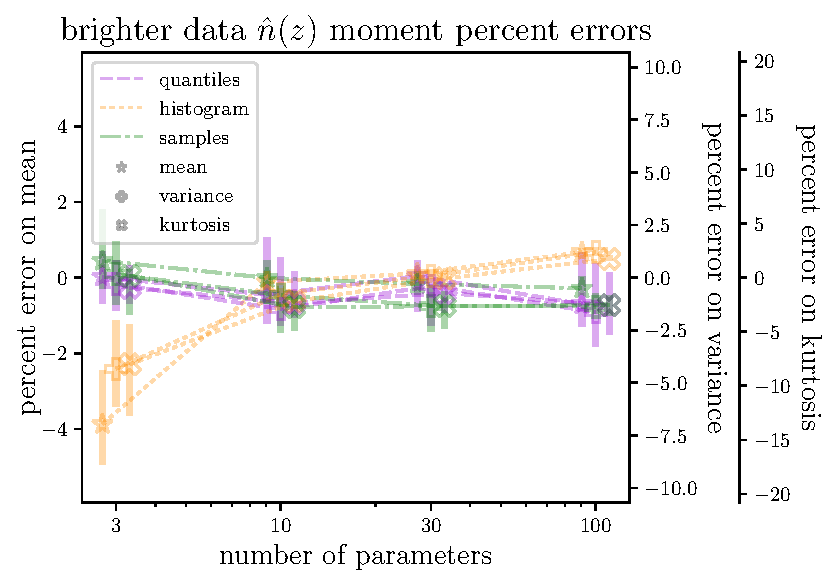
\includegraphics[width=\columnwidth]{graham_nz_err.pdf}    
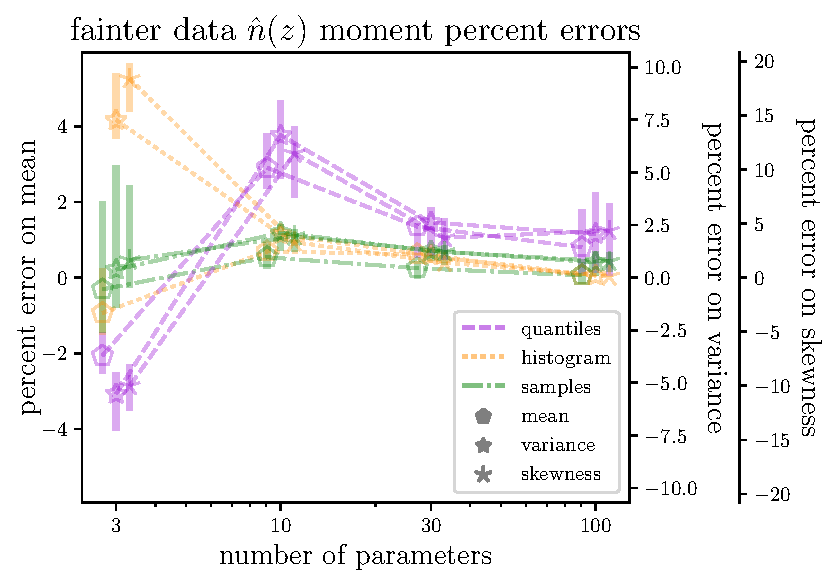
\includegraphics[width=\columnwidth]{schmidt_nz_err.pdf}
    \caption{
    The percent error on the mean ($\bigstar$), variance ($+$), and kurtosis 
($\times$) of the stacked estimator $hat{n}(z)$ of the redshift distribution 
for each dataset as a function of the number $N_{f}$ of stored parameters for 
the quantile (dashed purple line), samples (dash-dotted greenline), and 
histogram (dotted orangeline) formats with interquartile range error bars based 
on 10 instantiations of 100 galaxies, where the percent errors and their 
interquartile ranges are offset about $N_{f}$ to improve readability.
    Left panel: The \mgdata dataset shows evolution with $N_{f}$ of the 
$\hat{n}(z)$ moment percent errors for the histogram format but none for the 
samples and quantile formats.
    Right panel: The \ssdata dataset shows qualitatively different evolution 
with $N_{f}$ of the $\hat{n}(z)$ moment percent errors for the three formats 
and for each moment.
    \label{fig:nz_moment_errs}}
  \end{center}
\end{figure*}
In this metric, the significant impact of data properties is quite apparent.
To explain this, we draw the reader's attention to Figure~\ref{fig:stacked} and 
note that the actual redshift distribution for both datasets is similar, but 
the redshift range over which they are defined is larger for the \mgdata 
dataset than the \ssdata dataset.

In the \mgdata dataset, the evolution of the $\hat{n}(z)$ moment errors with 
$N_{f}$ differs for the histogram format relative to the samples and quantile 
formats; while the samples and quantile formats exhibit essentially no 
evolution in excess of the error bars between instantiations, the histogram 
format significantly underestimates the moments at low $N_{f}$, effectively 
approximates the moment errors at intermediate $N_{f}$, and overestimates them 
at high $N_{f}$.
For $N_{f}=3$, the moments are grossly underestimated because most of the 
probability density of $\hat{n}'(z)$ falls into the lowest single redshift bin 
(explaining the higher moments), and the lowest redshift bin has most of the 
probability density of $\hat{n}'(z)$ above the middle of the bin (explaining 
the mean).
When the bins are too small, at $N_{f}=100$, those at high redshifts have most 
of their probability density below the middle of the bin, leading to slightly 
overestimated moments.
Because the \pz s in the \mgdata dataset are so narrow and unimodal overall, 
the reconstructions of the samples and quantile parametrizations are highly 
accurate where most of the probability density is even with low $N_{f}$, so the 
$\hat{n}'(z)$ moments are consistently recovered to within $<1\%$.

In the \ssdata dataset, the issues are different because the redshift range of 
the original \pz s is smaller and the \pz s themselves are broader.
The samples format has no significant evolution in moment errors with $N_{f}$, 
the histogram format severely overestimates the higher moments at low $N_{f}$, 
and the quantiles format severely underestimates the moments at low $N_{f}$, 
severely overestimates them at intermediate $N_{f}$, and moderately 
overestimates them at high $N_{f}$.
The samples format may suffer from shot noise for broad, multimodal \pz s, but 
the result is just spikier \pz s that produce narrow features in $\hat{n}(z)$ 
that do not significantly affect the moments.
The histogram format's overestimation of higher moments at low $N_{f}$ in the 
\ssdata dataset is caused by the bulk of the probability density of 
$\hat{n}'(z)$ falling almost evenly into the two low redshift bins with far 
less probability in the highest bin.
As was hinted at in Figure~\ref{fig:kld_moments}, the quantile 
parametrization's \pz\ KLD distribution has large moments, and the KLD is most 
sensitive to a poor approximation of the tails of the distribution.
Both the underestimation of the $\hat{n}(z)$ moments at low $N_{f}$ and the 
overestimation of the $\hat{n}(z)$ moments at intermediate $N_{f}$ are due to 
the choice of a suboptimal reconstruction scheme for quantiles that could 
doubtlessly be improved in the future.
The quantile format's overestimation of the moments even at high $N_{f}$ can be 
explained by the fact that it is not limited to the redshift range over which 
the original \pz s were defined, a possible oversight of the \qp\ 
implementation; a broad \pz\ may be reconstructed with probability density 
outside the redshift range of the original \pz s and then truncated and 
normalized prior to stacking, and because broad \pz s are more likely to occur 
at high redshift, this excess probability is more likely to be at high 
redshift, slightly but consistently inflating the moments.


\section{Conclusions \& Future Directions}
\label{sec:conclusions}

This work develops a principled, systematic approach to choosing a 
parametrization for storing a catalog of \pz s from a survey of known data 
properties with a goal of balancing the available storage resources against the 
accuracy of the \pz s and science products thereof reconstructed from the 
stored parameters.
We demonstrate the recommended method on two realistic mock datasets 
representative of upcoming \pz\ catalogs and draw the following general 
conclusions:
\begin{itemize}
  \item Though the histogram format has the strongest presence in the 
literature, it generally has a higher loss of information and moment percent 
error of the reconstructed \pz s, except when a very large number of parameters 
are stored.
  \item The parametrization that best approximates individual \pz s may not be 
optimal for a given science metric.
  \item Increasing the number of stored parameters reduces the loss of 
information and percent error in the moments of the reconstructed \pz s, but 
the marginal improvement is not always significant.
  \item Some general trends are shared among the datasets we used in our tests, 
but much of the qualitative and quantitative behavior is different.
\end{itemize}
To be clear, we do not advocate for a one-size-fits-all solution to the problem 
of compressing \pz\ catalogs and emphasize that the optimal choice depends on 
the science metric(s) and characteristics of the data, and any decision should 
account for the absolute, relative, and marginal behavior of the formats 
considered as a function of the number of stored parameters.

Furthermore, though we discussed the previous use of each format in science 
calculations, we do not endorse the preference of any format on the basis of 
existing infrastructure for its use.
Rather, we anticipate great advances in the development of analysis techniques 
that best make use of the information in \pz s and encourage the community to 
then choose parametrizations that most effectively serve the needs of those 
intended practices.
Future analyses may also consider options we did not, such as new formats or 
the storage of different numbers of parameters for each galaxy in the catalog.

Given the constraint that LSST will be able to store only 200 floating point 
numbers to quantify the redshift of each galaxy and intends to include the 
results of several \pz\ codes, we can safely say that LSST can store the output 
of more than one \pz\ code without risk of significant loss of information.
Had our results indicated a significant reduction in KLD for a small increase 
in the number of stored parameters, we would present to decisio nmakers within 
the collaboration evidence in support of increasing that allocation.
So that decisions of this kind can be optimized for all future surveys, the 
\qp\ Python package developed for this project is made public on GitHub as a 
tool for use by the broader community.
We invite contributions of additional reconstruction schemes, formats, and 
metrics to the public GitHub repository.


\subsection*{Appendix}
\label{sec:kld}

We develop some intuition for the Kullback-Leibler Divergence by contrasting it 
with the familiar metric of the root-mean-square error (RMSE)
\begin{align}
  \label{eq:rmse}
  \mathrm{RMSE} &= \sqrt{\int (P(z) - \hat{P}(z))^{2} dz}.
\end{align}
Consider the simple example of a Gaussian $P(z)=\mathcal{N}(\mu_{0}, 
\sigma_{0}^{2})$ being approximated by a Gaussian $P'(z)=\mathcal{N}(\mu, 
\sigma^{2})$, whose KLD is
\begin{align}
  \label{eq:gaussian}
  \mathrm{KLD} &= 
\frac{1}{2}\left(\log\left[\frac{\sigma^{2}}{\sigma_{0}^{2}}\right] + 
\frac{\sigma_{0}^{2}}{\sigma^{2}} + \frac{(\mu-\mu_{0})^{2}}{\sigma^{2}} - 
1\right)
\end{align}
To get a sense of the units of information, we can calculate the KLD and RMSE 
in some limiting cases.
If $\sigma=\sigma_{0}$ but $\mu=\mu_{0}+1$, we obtain 
$\mathrm{KLD}=\frac{1}{2}$ nat -- if the mean of the approximation is wrong by 
an additive factor of $\sigma$, half a nat of information is lost.
If $\mu=\mu_{0}$ but $\sigma=\sqrt{2\pi}\sigma_{0}$, we find 
$\mathrm{KLD}\approx\frac{1}{2}$ nat -- half a nat of information is also lost 
if the variance of the approximation is off by a multiplicative factor of 
$2\pi$.

We can use the KLD to identify notions of imprecision and inaccuracy.
Intuitively, precision must be related to how close $\sigma$ is to $\sigma_{0}$ 
and accuracy must be related to how close $\mu$ is to $\mu_{0}$.

If $\mu\approx\mu_{0}$, we can say $\mathrm{KLD}\sim\log[r] + \frac{1}{2}r^{-2} 
- \frac{1}{2}$ where $r^{-1}\equiv\frac{\sigma_{0}}{\sigma}$ is a measure of 
\textit{precision}, whose behavior is illustrated in 
Figure~\ref{fig:precision}, alongside that of the RMSE.  We observe that an 
overestimated variance increases the KLD as the log of the square root of the 
ratio of the estimated variance to the true variance.

\begin{figure}
  \begin{center}
    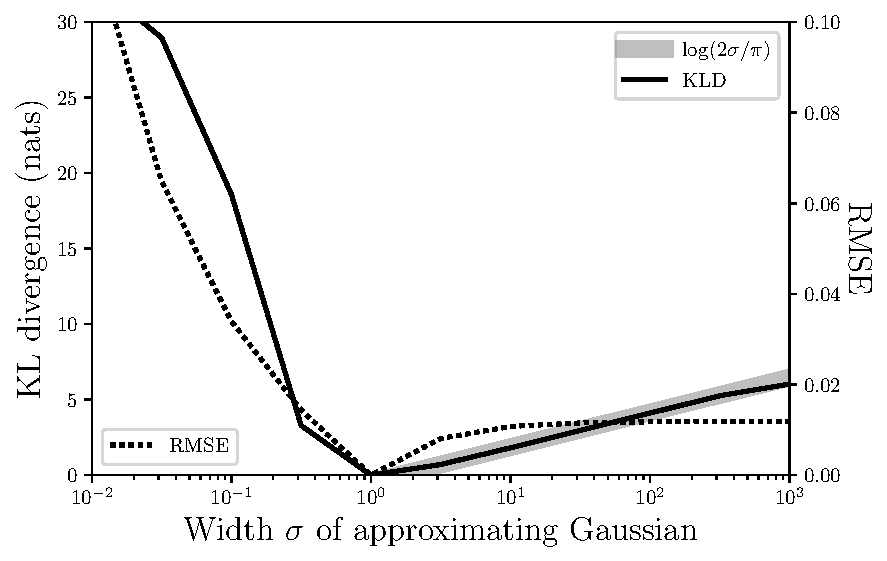
\includegraphics[width=\columnwidth]{figures/precision.pdf}
    \caption{The KLD (solid black line) is proportional to the log of the 
inverse precision $r$ for $\sigma>\sigma_{0}$, behavior that is qualitatively 
similar to that of the RMSE (dotted black line).
    \label{fig:precision}}
  \end{center}
\end{figure}

When $\sigma\approx\sigma_{0}$, $\mathrm{KLD}\sim t^{2}$ in terms of the 
\textit{tension} $t\equiv\frac{(\mu-\mu_{0})^{2}}{\sigma^{2}}$, whose 
concordance is illustrated in Figure~\ref{fig:tension}.  This behavior hints at 
the KLD's sensitivity to the tails of a distribution, relative to the RMSE, 
which does not continue increasing with tension.  The notion of tension may be 
more important for cosmological applications of \pz s, indicating the KLD is a 
more appropriate metric than the RMSE.

\begin{figure}
  \begin{center}
    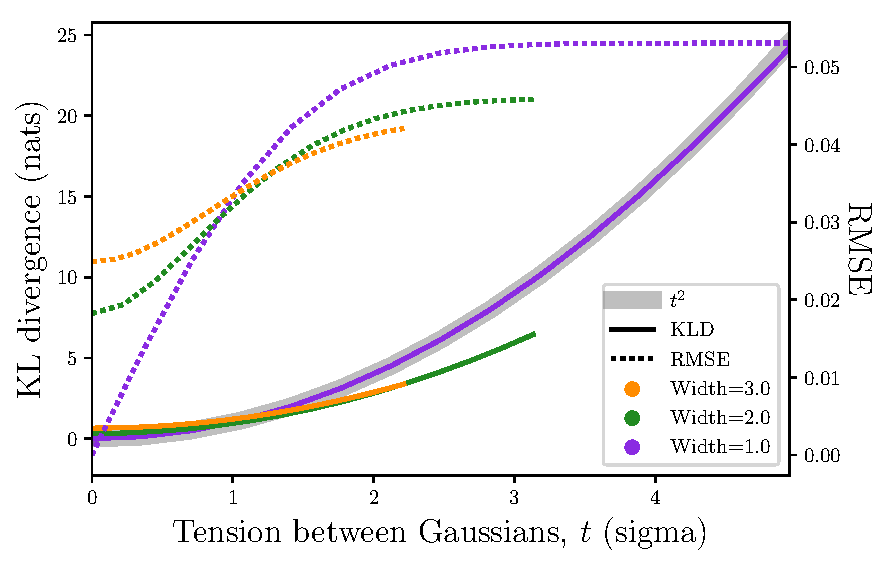
\includegraphics[width=\columnwidth]{figures/tension.pdf}
    \caption{The KLD (solid line) is equal to the square of the tension $t$, 
with a small additive offset when $r\neq1$, whereas the RMSE (dotted line) is 
relatively insensitive to tension past a certain point.
    \label{fig:tension}}
  \end{center}
\end{figure}

\subsection*{Acknowledgments}


This work was incubated at the 2016 LSST-DESC Hack Week hosted by Carnegie 
Mellon University.
The work of PJM was supported by the U.S. Department of Energy under contract 
number DE-AC02-76SF00515.
SJS was partially supported by the National Science Foundation under grant 
N56981CC.


%
%This is the text imported from \code{acknowledgments.tex}, and will be replaced by some standard LSST DESC boilerplate at some point.
%

We would like to thank the LSST-DESC Publications Board and review committee 
for helpful feedback on preparation of this paper.

Author contributions are listed below. \\
A.I.~Malz: Initiated project, led development work. \\
P.J.~Marshall: Advised on statistics, and project design and management. \\
S.J.~Schmidt: Produced the PDFs for the fainter mock catalog. \\
M.L.~Graham: Produced the photometry and PDFs for the brighter mock catalog. \\
J.~DeRose: Produced the photometry for the fainter mock catalog. \\
R.~Wechsler: Supervised production of the fainter mock catalog. \\



\bibliography{lsstdesc,main}

\end{document}
